%! Suppress = MightBreakTexify
\documentclass{article}

\usepackage[utf8]{inputenc}
\usepackage[pagebackref,citecolor=blue,linkcolor=OliveGreen,urlcolor=Mahogany,colorlinks]{hyperref}
\usepackage[usenames,dvipsnames]{xcolor}
\usepackage{url}
\usepackage{amsmath}
\usepackage{amsfonts}
\usepackage{lmodern}
\usepackage{etoolbox}
\usepackage{amsthm}
\usepackage{color}
\usepackage{cleveref}
\usepackage{tikz}
\usetikzlibrary{positioning}

% coq
\usepackage{minted}
\usemintedstyle{emacs}

\crefformat{section}{\S#2#1#3} % see manual of cleveref, section 8.2.1
\crefformat{subsection}{\S#2#1#3}
\crefformat{subsubsection}{\S#2#1#3}

\newcommand{\TODO}[0]{{\color{red} TODO}}
\newcommand{\lrangle}[1]{\langle #1\rangle}
\newcommand{\RedPRL}{{\color{red} Red}PRL}

\newdimen\mathindent\mathindent\leftmargini
\usepackage[links,references]{latex/agda}
\usepackage{newunicodechar}
\newunicodechar{λ}{\ensuremath{\mathnormal\lambda}}
\newunicodechar{←}{\ensuremath{\mathnormal\from}}
\newunicodechar{→}{\ensuremath{\mathnormal\to}}
\newunicodechar{↦}{\ensuremath{\mathnormal\mapsto}}
\newunicodechar{∀}{\ensuremath{\mathnormal\forall}}
\newunicodechar{≡}{\ensuremath{\mathrel{=}}}
\newunicodechar{β}{\ensuremath{\mathnormal\beta}}
\newunicodechar{Π}{\ensuremath{\mathnormal\Pi}}
\newunicodechar{ℕ}{\ensuremath{\mathnormal{\mathbb N}}}
\newunicodechar{ℤ}{\ensuremath{\mathnormal{\mathbb Z}}}
\newunicodechar{¹}{\ensuremath{\mathnormal{^1}}}
\newunicodechar{²}{\ensuremath{\mathnormal{^2}}}
\newunicodechar{∧}{\ensuremath{\mathnormal{\wedge}}}
\newunicodechar{∨}{\ensuremath{\mathnormal{̌\vee}}}



\title{Constructive Interpretations of HoTT (Draft)}
\author{Tesla Ice Zhang}

% allow multiple labels in displaymath
%! Suppress = Makeatletter
\makeatletter
\patchcmd{\mathdisplay}
{\let\label\label@in@display}{}
{}{\fail}
%! Suppress = Makeatletter
\makeatother

% new cmd
\newcommand\xtag{
\refstepcounter{equation}%
\;\;\text{(\theequation)}}
\newcommand{\refl}{\textsf{refl}}

\begin{document}
\maketitle

\tableofcontents

In the HoTT Book~\cite{hottbook},
the identity type is defined the same way as the one
in Martin-L\"{o}f Type Theory (hereafter as ``MLTT'')~\cite{MLTT},
but used differently (stated in Chapter 1 notes).
The elimination rule of the identity type is called \textbf{path induction},
but according to its definition we can tell
it's just another name of the MLTT \textbf J rule.

We distinguish them by calling the HoTT identity type the \textit{path type},
while the MLTT one as the \textit{identity type}.
The most notable difference is that the path type is
\textit{proof relevant} (implies the absence of
\textit{Axiom K}~\cite{AxiomK}).

By not providing a better definition of the path type,
we have to assume function extensionality as an axiom,
and we cannot compute transport on nontrivial paths.

To safely assume the univalence axiom, we need to avoid having Axiom K
in our type system.
Agda~\cite{Agda} implements~\cite{WithoutK} this via a flag \texttt{--without-K},
while in Coq~\cite{Coq}, Axiom K is not assumed.
Agda have further developed to have a without-K-compatible \textsf{Prop}
universe~\cite{PropWithoutK}, a without-K-compatible definitional equality
customization strategy~\cite{RewriteWithoutK}, and many other stuffs.
Another dependently-typed programming language similar to Agda,
Idris~\cite{Idris}, sticks to Axiom K and is
inconsistent~\cite{IdrisHoTT} with the univalence axiom.

Even we have ways to avoid Axiom K,
we are still missing a constructive version of function extensionality,
and we also cannot compute the univalence axiom.

\subsection{Introduction}
\label{subsec:introduction}

This note is about giving HoTT a completely constructive interpretation,
from an implementation and user-experience perspective.
The categorical models behind are discussed only when necessary.

By giving a constructive interpretation of HoTT,
these issues are addressed:

\begin{itemize}
\item The path type should be constructive --
  there need to be formation, introduction and
  elimination rules (\cref{sec:path}).
\item Transport should compute (\cref{subsec:coe}).
\item The univalence axiom (\cref{sec:ua}) and function extensionality
  (\cref{subsec:path-prop}) should compute.
\item Inductive types~\cite{Inductive} should allow \textbf{path constructors}
  to form \textit{higher inductive types} (\cref{sec:hit}).
\end{itemize}

This note assumes the reader to:

\begin{itemize}
\item Have brief understanding of HoTT.
\item Have basic understanding of dependent type programming and MLTT.
\end{itemize}
To define Path constructively,
we may get some inspiration from its topological definition.
Open-up the \href{https://ncatlab.org/nlab/show/path}{``path'' segment in nLab},
there is a mathematical definition of a path, written as:

\[
  \mathbb I \rightarrow X
  \xtag
\]

Topologically, a path in a space $X$ is a continuous map
from an interval (denoted $\mathbb I$) to $X$.
Type theoretically, $\mathbb I$ and $X$ are types,
and $\mathbb I \rightarrow X$ is a function type from $\mathbb I$ to $X$.
As paths represent a relation \textit{between} two terms
(endpoints, but type theoretically),
these two terms should show up in the path type as well
(similar to MLTT identity type).
Therefore the formation rule for path types is naturally:

\[
  \cfrac{
    \Gamma \vdash X \ \textbf{type}
    \quad
    \Gamma \vdash a : X
    \quad
    \Gamma \vdash b : X
  }{\Gamma \vdash a =_X b \ \textbf{type}}
  \xtag
\]

Up to the time where this note is written,
everyone tries to define constructive HoTT defines path types this way.
They have different introduction and elimination rules,
but all of their introduction rules are
based on the interval type $\mathbb I$
and the elimination rules are slimiar to function application.

We can also define heterogeneous path types
(path between two terms of different types)
by changing the type $X$ into a type family $f$,
indexed by the interval type $\mathbb I$,
to allow paths between terms of different types:

\[
  \cfrac{
    \Gamma \vdash X \ \textbf{type}
    \quad
    \Gamma \vdash a : X
    \quad
    \Gamma \vdash b : X
    \quad
    \Gamma \vdash f : \mathbb I \rightarrow X
  }{\Gamma \vdash a =_f b \ \textbf{type}}
  \xtag
\]

\subsection{Interval types}

The interval type has very simple formation rule
and introduction rule:

\[
  \vdash \mathbb I\ \textbf{type}
  \xtag \quad
  \vdash \textsf 0 : \mathbb I
  \xtag \quad
  \vdash \textsf 1 : \mathbb I
  \xtag
\]

The programming language Arend~\cite{Arend} uses a different notation
(\textsf{left} instead of \textsf 0, \textsf{right} instead of \textsf 1)
for interval endpoints.
We will still use \textsf 0 and \textsf 1 when talking
about Arend for consistency.

The interval type do not yet have an elimination rule,
so we cannot have a predicate on an interval.

By this definition of interval, the path type can
have the following introduction rule
(definitional equality between term $a$ and $b$
is denoted as $a \equiv b$,
usually implemented via conversion checking or normalization):

\[
  \cfrac{
    \Gamma \vdash a =_X b \ \textbf{type}
    \quad
    \Gamma, i : \mathbb I \vdash t : X
    \quad
    (\lambda i. t) \ \textsf 0 \equiv a
    \quad
    (\lambda i. t) \ \textsf 1 \equiv b
  }{
    \Gamma \vdash \lrangle i t : a =_X b
  }
  \xtag
\]

Heterogeneously:

\[
  \cfrac{
    \Gamma \vdash a =_F b \ \textbf{type}
    \quad
    \Gamma, i : \mathbb I \vdash t : F \ i
    \quad
    (\lambda i. t) \ \textsf 0 \equiv a
    \quad
    (\lambda i. t) \ \textsf 1 \equiv b
  }{
    \Gamma \vdash \lrangle i t : a =_F b
  }
  \xtag
\]

The above definition is used in Cubical Type Theory~\cite{CCHM,CHM}
(hereafter as CTT), Cartesian Cubical Type
Theory~\cite{CCTT,CCTT2,CHTT} (hereafter as CCTT).
There are three usable implementations of CTT described in~\cite{CHM},
including cubicaltt~\cite{CubicalTT},
mlang~\cite{Mlang} and Cubical Agda~\cite{CubicalAgda}.
For CCTT, there are two, including
redtt~\cite{RedTT} and yacctt~\cite{YaccTT},
which implement different variations of CCTT.

The syntax is intentionally made similar to a lambda abstraction,
as the introduction rule is the same as lambda abstraction with
additional two definitional equalities required.
The elimination rule for a path is therefore similar to an application,
with two additional reduction rules -- applying an interval $i$ to
an arbitrary term whose type is known to be a path type $a =_X b$
will reduce to $a$ if $i \equiv \textsf 0$ or $b$ if $i \equiv \textsf 1$:

\[
  \cfrac{
    \Gamma \vdash p : a =_X b
  }{
    \Gamma \vdash p\ \textsf 0 \equiv a
    \quad
    \Gamma \vdash p\ \textsf 1 \equiv b
  }
  \xtag \label{eqn:path-app}
\]

Rule~\ref{eqn:path-app} holds even if $p$ is a neutral term,
or a contructor (in case there's path constructors,
introduced in~\cref{sec:hit}).
Therefore constructor application can be redex as well.

CTT and CCTT (and many other variations) have different primitive
operations defined for the interval type,
we discuss this later in~\cref{sec:kan}.

Arend on the other hand defines a primitive operator \textsf{path}
as the introduction rule for path:

\[
  \cfrac{
    \Gamma \vdash X \ \textbf{type}
    \quad
    \Gamma \vdash t : \mathbb I \rightarrow X
  }{
    \Gamma \vdash \textsf{path} \ t : (t \ \textsf 0) =_X (t \ \textsf 1)
  }
  \xtag
\]

The elimination of paths is still similar to CTT or CCTT.

CTT and CCTT do not support creating paths between intervals,
while Arend do.
Thus the following judgement holds in Arend, say,
that there exists a path between \textsf 0 and \textsf 1:

\[
  \vdash \textsf{path}\ (\lrangle i i) : \textsf 0 =_{\mathbb I} \textsf 1
  \xtag \label{eqn:0-1-arend}
\]

This does not mean that \textsf 0 is identical to \textsf 1.
They are not equivalent definitionally, but propositionally.
Here's the concrete syntax of~\ref{eqn:0-1-arend} in Arend:

\begin{minted}{arend-lexer.py:ArendLexer -x}
  \func interval-path : left = right => path (\lam i =>  i)
\end{minted}

\subsection{Path properties}
\label{subsec:path-prop}
\input{latex/path-properties}

\subsection{Transport}
\label{subsec:coe}

The idea of \textit{type-safe coercion} is like
casting a variable of type $A$ to type $B$ by providing a proof
of $A =_{\mathcal U} B$:

\[
  \textsf{coe} : A =_{\mathcal U} B \rightarrow A \rightarrow B
  \xtag \label{eqn:coe-a-b-id}
\]

Bringing in the idea of path types,
assuming $p : A =_{\mathcal U} B$, by~\ref{eqn:path-app}
we know that $p \ \textsf 0 \equiv A$ and
$p \ \textsf 1 \equiv B$,
so~\ref{eqn:coe-a-b-path} is effectively the same
as~\ref{eqn:coe-a-b-id}:

\[
  \textsf{coe} : (p : A =_{\mathcal U} B) \rightarrow p \ \textsf 0
  \rightarrow p \ \textsf 1
  \xtag \label{eqn:coe-a-b-path}
\]

The return type of \textsf{coe} can be generalized over
the interval on the input path:

\[
  \textsf{coe} : (p : A =_{\mathcal U} B) \rightarrow p \ \textsf 0
  \rightarrow (i : \mathbb I) \rightarrow p \ i
  \xtag \label{eqn:coe-a-b-path-gen}
\]

\ref{eqn:coe-a-b-path-gen} is known as the ``generalized transport''
operation, denoted as \textsf{coe} in Arend and CCTT,
and \AgdaFunction{transp} in CTT.
We use \textsf{coe} to refer to this general concept for consistency.
And by the way,
Arend's \textsf{coe} takes function over interval instead
of a path as its first argument:

\[
  \textsf{coe} : (p : I \rightarrow \mathcal U)
  \rightarrow p \ \textsf 0
  \rightarrow (i : \mathbb I) \rightarrow p \ i
  \xtag
\]

Right now there is neither nontrivial path nor path on types,
while transport along identity paths is just a fancy version
of the identity function, thus we do not need to worry about the
computation of \textsf{coe} yet.
We further discuss \textsf{coe} in~\cref{sec:ua}.

In CTT and CCTT, we cannot transport along paths between paths,
but it's not the case in Arend.
Arend uses \textsf{coe} to prove path symmetry and transitivity.
Here's a proof, assuming three inhabitants $a, b, c$ of type $A$
and the trivial path $\refl_a : a =_A a$:

\[
  \cfrac{
    \Gamma \vdash p : a =_A b
  }{
    \Gamma \vdash (\textsf{coe}
    (\lambda i. (p\ i =_A a)) \ \refl_a \ \textsf 1)
    : b =_A a
  }
  \xtag \label{eqn:arend-proof-sym}
\]

% Note that in Arend's concrete syntax, path application is not
% $p\ i$ but $p\ @\ i$ and lambda abstraction is not $\lambda x.y$ but
% $\backslash{}\textsf{lam} \ x \Rightarrow y$.
The Arend's concrete syntax of~\ref{eqn:arend-proof-sym} is:

\begin{minted}{arend-lexer.py:ArendLexer -x}
  \func sym {A : \Type} {a b : A} (p : a = b) : b = a =>
    coe (\lam i => p @ i = a) idp right
\end{minted}

What happened in~\ref{eqn:arend-proof-sym} is that we transported
along the following interval lambda:

\[
  f = \lambda i. (p\ i =_A a)
  \xtag
\]

As $p : a =_A b$, we have
$(f \ \textsf 0) \equiv (p \ \textsf 0 =_A a) \equiv (a =_A a)$ and
$(f \ \textsf 1) \equiv (p \ \textsf 1 =_A a) \equiv (b =_A a)$,
so $f$ is similar to a path $(a =_A a) =_{\mathcal U} (b =_A a)$.
By providing a proof \refl of $a =_A a$,
we obtain the proof of the right hand side of $f$, which is $b =_A a$.
The proof of transitivity is similar, as in~\ref{eqn:arend-proof-trans}.
Analyzing how it works is left as an exercise.

\[
  \cfrac{
    \Gamma \vdash p : a =_A b
    \quad
    \Gamma \vdash q : b =_A c
  }{
    \Gamma \vdash (\textsf{coe}
    (\lambda i. (a =_A q\ i)) \ p \ \textsf 1)
    : a =_A c
  }
  \xtag \label{eqn:arend-proof-trans}
\]

It looks like the following in Arend:

\begin{minted}{arend-lexer.py:ArendLexer -x}
  \func trans {A : \Type} {a b c : A}
              (p : a = b) (q : b = c) : a = c =>
    coe (\lam i => a = q @ i) p right
\end{minted}

\subsection{Homotopies}
\label{subsec:hom}

\TODO

By the above constructive path type,
we can extend inductive types with path constructors.
Recall that a constructor of an inductive type $T$ is
similar to a function whose return type is $T$,
but does not reduce.

Inductive types with path constructors are called
\textit{higher inductive types} (hereafter as HIT),
which is discussed in Chapter 6 of the HoTT Book.
The integer type $\mathbb Z$ is a good example of HIT.
Given this natural number $\mathbb N$ definition:

\[
  \vdash \mathbb N \ \textbf{type}
  \xtag
\]
\[
  \vdash \textsf{zero} : \mathbb N
  \xtag
  \quad
  \vdash \textsf{succ} : \mathbb N \rightarrow \mathbb N
  \xtag
\]

We can derive the definition of $\mathbb Z$:

\[
  \vdash \mathbb Z \ \textbf{type}
  \xtag
\]
\[
  \vdash \textsf{pos} : \mathbb N \rightarrow \mathbb Z
  \xtag
  \quad
  \vdash \textsf{neg} : \mathbb N \rightarrow \mathbb Z
  \xtag
\]
\[
  \vdash \textsf{zro} :
  \textsf{pos zero} =_{\mathbb Z} \textsf{neg zero}
  \xtag
\]

$\mathbb Z$ has two \textbf{point constructors}
\textsf{pos} and \textsf{neg}, with one \textbf{path constructor}
\textsf{zro} whose two endpoints are \textsf{pos zero} and \textsf{neg zero}.

Path constructors add constraints to the operations defined on HITs.
Taking the $\mathbb Z$ type as an example,
for an arbitrary type $A$ and a function $f : \mathbb Z \rightarrow A$,
the path $p = \textsf{ap}_f(\textsf{zro})$ should to some extent
satisfy the following two equalities
(some model require these equalities to be definitional, some don't):

\[
  p\ \textsf 0 =_A f\ (\textsf{pos zero})
  \xtag
  \quad
  p\ \textsf 1 =_A f\ (\textsf{neg zero})
  \xtag
\]

For the general case, given arbitrary HIT $T$, an arbitrary type $A$ and
function $f : T \rightarrow A$, for all path constructors
$p : a =_T b$ of $T$, there should be:

\[
  p\ \textsf 0 =_A f\ a
  \xtag
  \quad
  p\ \textsf 1 =_A f\ b
  \xtag
\]

We call this property ``agree on path constructors'',
or ``respect the path constructors''.

Higher inductive types are similar in CTT and CCTT,
while Arend is somehow different from the other two.

\subsection{Axiomatic approach}

In the old days, there were no constructive path type.
People use the MLTT identity type and
work with HITs by postulating their existence.
What they're actually postulating is the existence of the path constructors.

There had been a lot of work done based on this approach,
under various proof assistants such as Hoq
(a modified version of Coq, short for HoTT-Coq),
% TODO: is lean based on this?
and Agda (before cubical).

Many HITs can be generalized as a specialized version of a standard
quotient type. If we only postulate a quotient type, we can specialize
it into a number of other HITs to avoid postulating things again.

In the HoTT library~\cite{HottCoq} of Coq, the comments in the quotient
type module provide an ideal syntax for the quotient type definition:

\begin{minted}{coq}
  Inductive quotient : Type :=
  | class_of : A -> quotient
  | related_classes_eq : forall x y,
      (R x y), class_of x = class_of y
  | quotient_set : IsHSet quotient.
\end{minted}

We can read it as ``\textsf{quotient} is a type,
which has a point constructor \textsf{class\_of},
a path constructor \textsf{related\_classes\_eq}
and a proof that \textsf{quotient} is an HSet
(which is also a path constructor)''.
The \href{https://github.com/HoTT/HoTT/blob/b20bb573739284349a968bb219405255c744049d/theories/HIT/quotient.v#L40-L42}
{actual definition}, on the other hand, is:

\begin{minted}{coq}
  Private Inductive quotient
      {sR: is_mere_relation _ R} : Type :=
  | class_of : A -> quotient.
  Axiom related_classes_eq : forall {x y : A}, R x y ->
      class_of x = class_of y.  
  Axiom quotient_set : IsHSet (@quotient sR).
\end{minted}

We can read it as ``\textsf{quotient} is a type paramterized by a relation \textsf R,
and we postulate that the terms belonging to the same equivalent class are equivalent,
and we postulate that \textsf{quotient} is an HSet''.
This axiomatic definition does not ensure that functions defined on
axiomatic HITs agree on their path constructors.
In fact, it doesn't even ensure that terms belonging to the same equivalent
class are equivalent.

\input{latex/hit-agda-old}

\subsection{Conditions}
\label{subsec:conditions}

Arend supports two ways of defining HITs.
One is like Agda's old approach, say, providing path constructors
as something similar to a rewriting rule, namely \textit{conditions}.
They also support CCTT-style HITs, we talk about that together with
CCTT in~\cref{subsec:path-hit}.
However, Arend requires operations defined on HITs to agree on the conditions,
thus it's more consistent to the theoretical model of HITs in HoTT.

For instance, the integer type in Arend can be defined as:

\begin{minted}{arend-lexer.py:ArendLexer -x}
  \data Int
    | pos Nat
    | neg Nat \with {
      | zero => pos zero
    }
\end{minted}

Note that the constructor \textsf{neg} is attached with an additional
condition, saying that when the parameter of
\textsf{neg} appears to be \textsf{zero},
the term constructed by \textsf{neg} in this case should be
(definitionally) equivalent to \textsf{pos zero}.

Consider the following function, which do not agree with this condition:

\begin{minted}{arend-lexer.py:ArendLexer -x}
  \func absolute-value-bad (x : Int) : Nat
    | pos n => suc n
    | neg n => n
\end{minted}

When checking the \textsf{neg} clause, Arend substitutes $n$ with
\textsf{zero} according to the condition, and check if the returned
term, \textsf{zero}, is identical to
\textsf{absolute-value (pos zero)}, which reduces to \textsf{suc zero}.
It seems not, so the function is ill-formed.
Changing the definition to the following will satisfy Arend:

\begin{minted}{arend-lexer.py:ArendLexer -x}
  \func absolute-value-good (x : Int) : Nat
    | pos n => n
    | neg n => n
\end{minted}

This one will also work, because both sides of the condition
are \textsf{suc zero}
(the function name \textsf{absolute-value} indicates that it's finding
the absolute value of the input integer, while the following function
is not actually doing that.
Thus we add the postfix \textsf{-cheat} to it):

\begin{minted}{arend-lexer.py:ArendLexer -x}
  \func absolute-value-cheat (x : Int) : Nat
    | pos n => suc n
    | neg n => suc n
\end{minted}

% The path constructors encoded as conditions
% are still so different from the point constructors.
% They are not listed along with other constructors,
% and when pattern matching against an \textsf{Int},
% only \textsf{pos} and \textsf{neg} are covered.

Conditions are simple, because they're just constraints.
A problem is that when defining operations on condition-based HITs,
the constraints added by conditions should hold definitionally.
In case of the \textsf{absolute-value} function,
$\textsf{absolute-value}(\textsf{neg zero}) \equiv
\textsf{absolute-value}(\textsf{pos zero})$ should hold definitionally.
There are times when definitional equalities are difficult to have,
so conditions may not be the ultimate solution.

As path constructors are called ``constructors'',
we'll have to define them as constructors anyway.

% To form more complicated path constructors
% (which cannot be expressed as a condition),
% we'll need to define the path constructors as constructors explicitly.
% There is a more fancy way to define path constructors,
% that is, to define them as constructors.

\input{latex/hit-agda-new}

\subsubsection{Another syntax}

In Arend (also in \RedPRL\ and redtt),
path constructors are not written as a constructor but of a path type.
Instead,

\TODO


\section{Kan operations}
\label{sec:kan}

In~\cref{subsec:coe}, we have seen an operation on paths,
that is \textsf{coe}, which returns a path~\footnote
{It's not actually a path in Arend, but a function over intervals.
  We can say it's \textit{almost} a path.}.
Since it returns a path, we may wonder how is the returned path
represented internally.
Ideally, we want \textsf{coe} to be a built-in but reducible function,
which means that it \textbf{computes} when fully applied.
Unfortunately, \textsf{coe} in Arend only computes in certain hard-coded cases,
which is not ideal.
There is a more general operation in CTT and CCTT which allows computation
on path operations, namely \textit{Homogenous composition}.

The idea is in one sentence:

\begin{displayquote}
  For any n-dimensional cube, it has $2 \times n$ faces.
  If we can construct $2 \times n - 1$ of them,
  the last one face can be obtained by doing a homogenous composition.
\end{displayquote}

In case it's two-dimensional, the cube becomes a square,
and it has four faces, which are all one-dimensional paths.
If we can have three of these paths,
we can obtain the last path via homogenous composition.
We can graph this process, as in~\cref{fig:simple-comp}
(assuming $\vdash a, b, c, d : A$).

\begin{figure}
\begin{center}
  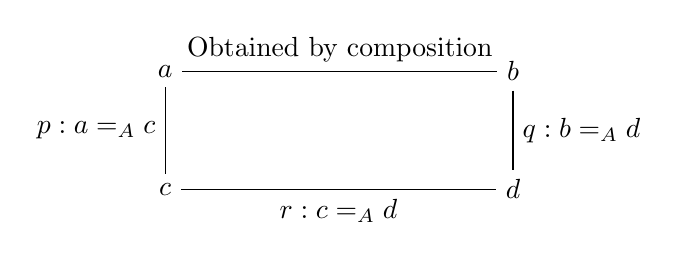
\begin{tikzpicture}[node distance=1.5cm]
    \node(1) {$a$};
    \node(2) [right=4cm of 1] {$b$};
    \node(4) [below of=1] {$c$};
    \node(3) [below of=2] {$d$};
    \draw (1) -- (2) node[midway,above] {Obtained by composition};
    \draw (1) -- (4) node[midway,left ] {$p : a =_A c$};
    \draw (3) -- (4) node[midway,below] {$r : c =_A d$};
    \draw (2) -- (3) node[midway,right] {$q : b =_A d$};
  \end{tikzpicture}
\end{center}
\caption{Simple composition}
\label{fig:simple-comp}
\end{figure}

This looks very similar to~\cref{fig:filler}
if we substitute $a$ with $b$ and $b, c, d$ with $a$.
We can also prove path composition by substituting $a$ with $c$.

Here's the surface syntax of homogenous composition.
In~\cite{CCHM}, there are two basic structures that the composition operation
is based on:

\begin{align*}
  \varphi &= (i=\textsf 0) \mid (i=\textsf 1)
  & \xtag \\
  u &= [ \; \varphi_1 \mapsto t_1,
      \dots, \varphi_n \mapsto t_n \; ]
  & \xtag
\end{align*}

$\varphi$ is called the \textit{Face lattice},
which stands for a constraint that specifies a face.
$u$ is a list of face-term pair $\varphi \mapsto t$,
where each pair specifies a term $t$ for a face $\varphi$.
Thus we can describe an open shape via $u$.

The composition operation is defined as following:

\newcommand{\comp}{\textsf{comp}}

\[
  \cfrac
  {\Gamma, i : \mathbb I \vdash A \quad
    \Gamma, \varphi, i : \mathbb I \vdash u : A \quad
    \Gamma \vdash a_0 : A(\textsf 0)[ \varphi \mapsto u(\textsf 0) ]}
  {\Gamma \vdash \comp^i~A~[ \varphi \mapsto u ]~a_0 :
    A(\textsf 1)[ \varphi \mapsto u(\textsf 1) ]}
\]

In naturally language, given
$A$ -- a type indexed by $\mathbb I$,
$a_0$ -- a term for the bottom face of the cube,
$u$ -- a list of face-term pairs representing all the faces except
$a_0$ and the top-missing face.
Then, $\comp^i~A~[ \varphi \mapsto u ]~a_0$ produces the top face.

In CCTT, there is another variation of $\varphi$:

\[
  \varphi = \dots \mid (i = j)
  \xtag
\]

This face specifies a diagonal,
giving us more computation rules.

\section{Univalence}
\label{sec:ua}

\TODO


\bibliography{ref}
\bibliographystyle{alpha}

\end{document}
